\section{Results - Enceladus \label{sec:results_Enceladus}}

\begin{figure*}[!t]
    \centering
    \begin{subfigure}[t]{0.9\linewidth} % contains the two plots in a single figure
        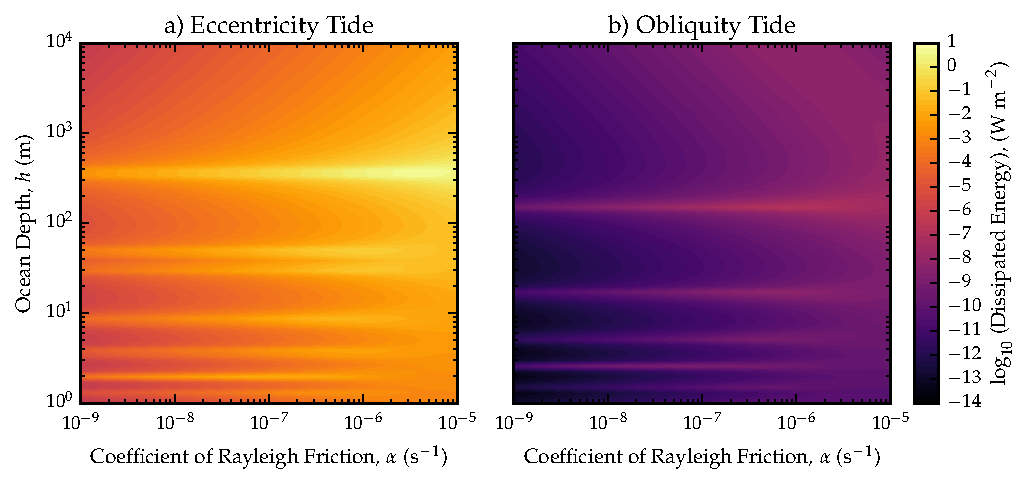
\includegraphics[width=\linewidth]{Figures/enceladus_linear}
        \phantomcaption
        \label{fig:lincEccEncel}
    \end{subfigure}
    \begin{subfigure}[t]{0\linewidth} % the hidden unwanted image
         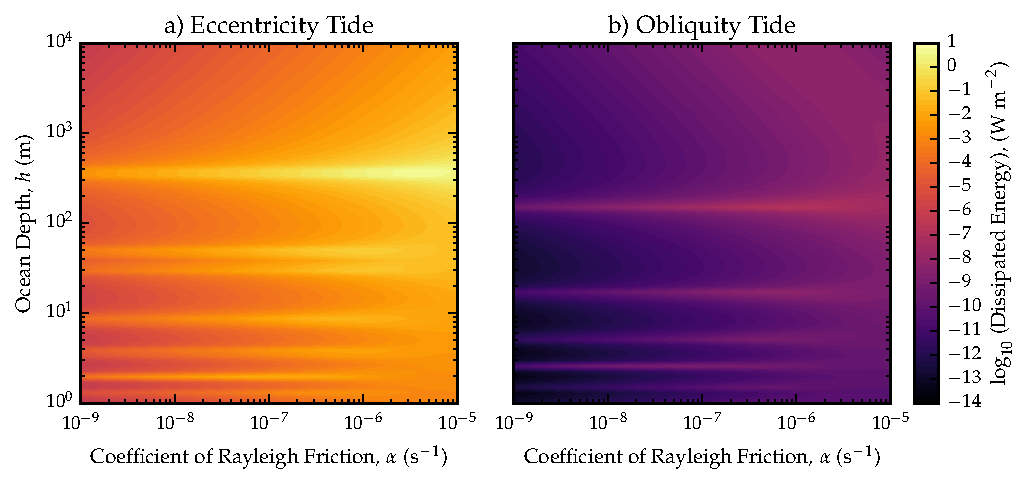
\includegraphics[width=\linewidth]{Figures/enceladus_linear}
         \phantomcaption
         \label{fig:linObliqEncel} 
    \end{subfigure}
    \vspace{-0.5cm}
\caption{Numerical global surface ocean dissipation solution for Titan under the eccentricity and obliquity tides. The logarithm of dissipated energy is shown as function of ocean depth, $h$, and Rayleigh friction coefficient, $\alpha$, on the left hand side of the figure. The numerical error for each tidal component is then shown in the right hand plots. All simulations were performed with $\ang{2}$ grid spacing. \label{fig:linEncel}}
\end{figure*}

\subsection{Implications for Enceladus}

\section{Scaling Laws \label{subsec:scaling}}